% !TeX root = proposal.tex
\chapter{Proposed Work}
In this chapter, we discuss our proposed work focusing on evaluating the user experience of the privacy-setting interface

To further explore this trade-off between parsimony and accuracy, and also to evaluate the usability of the proposed privacy-setting interface prototypes in~\cite{he2018data}, we are in a process of developing a user study to test these interface prototypes. This is going to be a between-subject study. All the participants will be recruited through Amazon Mechanical Turk. 

In this user study, we will manipulate two different independent variables to compare several default/profile solutions. The first one is the extend of default/profile's conservatives. We consider the default settings that with all disabled by default as the most conservative profile; and the default settings with all enabled by default as the most open profile, the `smart default' and `smart profiles' are considered to be in the middle. The other independent variable is the different levels of complexity for the settings interface. Hence 4x2=8 total experimental conditions (i.e., user interfaces) will be presented to the participants. The Dependent variable of our study will be the user experience of the system, including the satisfaction and trust to the company.

During the user study, the users will be first introduced the concept of the devices that appearing in the study, corresponding to the `Who' and `What' parameters of an IoT scenario. The introduction contains both figures, text, and audio information. After the introduction, the participant will be given an example scenario to further understand the context of our study. Attention checks will also be given here to make sure the participants have paid attention to the explanations.

After above procedures, one of the 8 user interfaces will be randomly chosen for each participants. Participants need to go through the whole interface to see if the preset privacy settings is suitable for them, and make necessary changes to accommodate their actual privacy demands. All these changes will be recorded to compared with the preset settings for further analysis purpose.

Next, the participants will be give a survey containing questions about three different aspects: \textit{Subjective System Aspects}, \textit{Personal Characteristics}, and \textit{Situational Characteristics}, as shown in Figure~\ref{fig:model}.

\begin{figure}
	\centering
	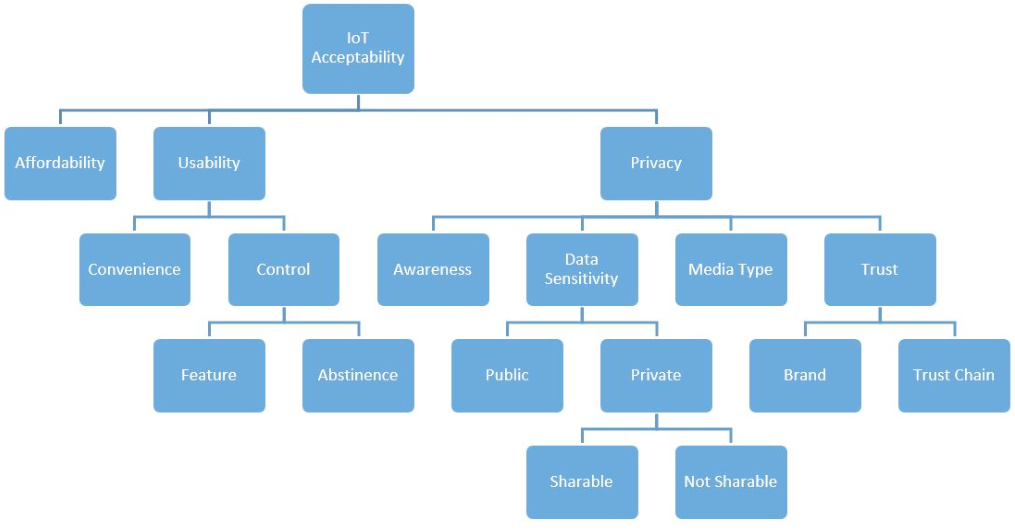
\includegraphics[width=0.48\textwidth]{figures/model.pdf}
	\caption{Accuracy of our clustering approaches}
	\label{fig:model}
\end{figure}

We expect to see a significant improvement for the `smart default' and `smart profile' interfaces in terms of system satisfaction and Trust over the baseline user interface (All-on or All-off). We will use statistics to analysis the effect of the independent variables on the subjective system aspects, and further mediation effect on the user experience. We also wonder how the personal characteristics ans situational characteristics affect the user experience. Finally, we will apply machine learning techniques to uncover deep insights of the results.